\documentclass[a4paper,10pt,oneside]{article}
\usepackage[polutonikogreek,italian]{babel}
\usepackage[utf8x]{inputenc}
\usepackage{amsmath}
\usepackage{amsthm}
\usepackage{amssymb}
\usepackage{amscd}
\usepackage{graphicx}
\usepackage{float}
\usepackage{array}
\usepackage{rotating}
\usepackage[small]{caption}
\usepackage{lscape}
\usepackage{fancybox}
\usepackage{booktabs}
\usepackage{exercise}
\parindent0ex
\usepackage{subfigure}
\renewcommand{\fboxsep}{0.4cm}
\usepackage{hyperref}
\renewcommand{\textfraction}{0.05}
\renewcommand{\topfraction}{0.95}
\renewcommand{\bottomfraction}{0.95}
\renewcommand{\floatpagefraction}{0.35}
\renewcommand{\ExerciseName}{Esercizio}
\renewcommand{\AnswerName}{Soluzione}
\renewcommand{\AnswerListName}{Soluzione}
\renewcommand{\ExerciseListName}{Es}
\setcounter{totalnumber}{5}
\newtheorem{definition}{Definizione}
\newtheorem{regola}{Regola}
\restylefloat{figure}
\begin{document}
\section*{Vettori}

\begin{definition}[Definizione operativa di vettore]
Diremo che una grandezza fisica è vettoriale se:
\begin{itemize}
 \item la somma rispetta la legge del parallelogrammo
 \item è possibile individuare un modulo, una direzione ed un verso per la grandezza
\end{itemize}
\end{definition}
\begin{definition}
Chiameremo versore un vettore di modulo unitario e lo indicheremo con: $\hat{\mathbf{x}}$, che leggeremo ``x cappuccio''
\end{definition}

\begin{regola}[Modulo di un vettore]
 Indicheremo il modulo di un vettore utilizzando le sbarre verticali: $|\mathbf{a}|$. Il modulo o lunghezza di un vettore si può determinare con il teorema di Pitagora, detti $a_x$ ed $a_y$ le proiezioni del vettore $\mathbf{a}$ sugli assi di un sistema cartesiano ortonormale risulterà:
\begin{equation*}
 |\mathbf{a}|=\sqrt{a_x^2+a_y^2}
\end{equation*}
\end{regola}


\begin{figure}[H]
 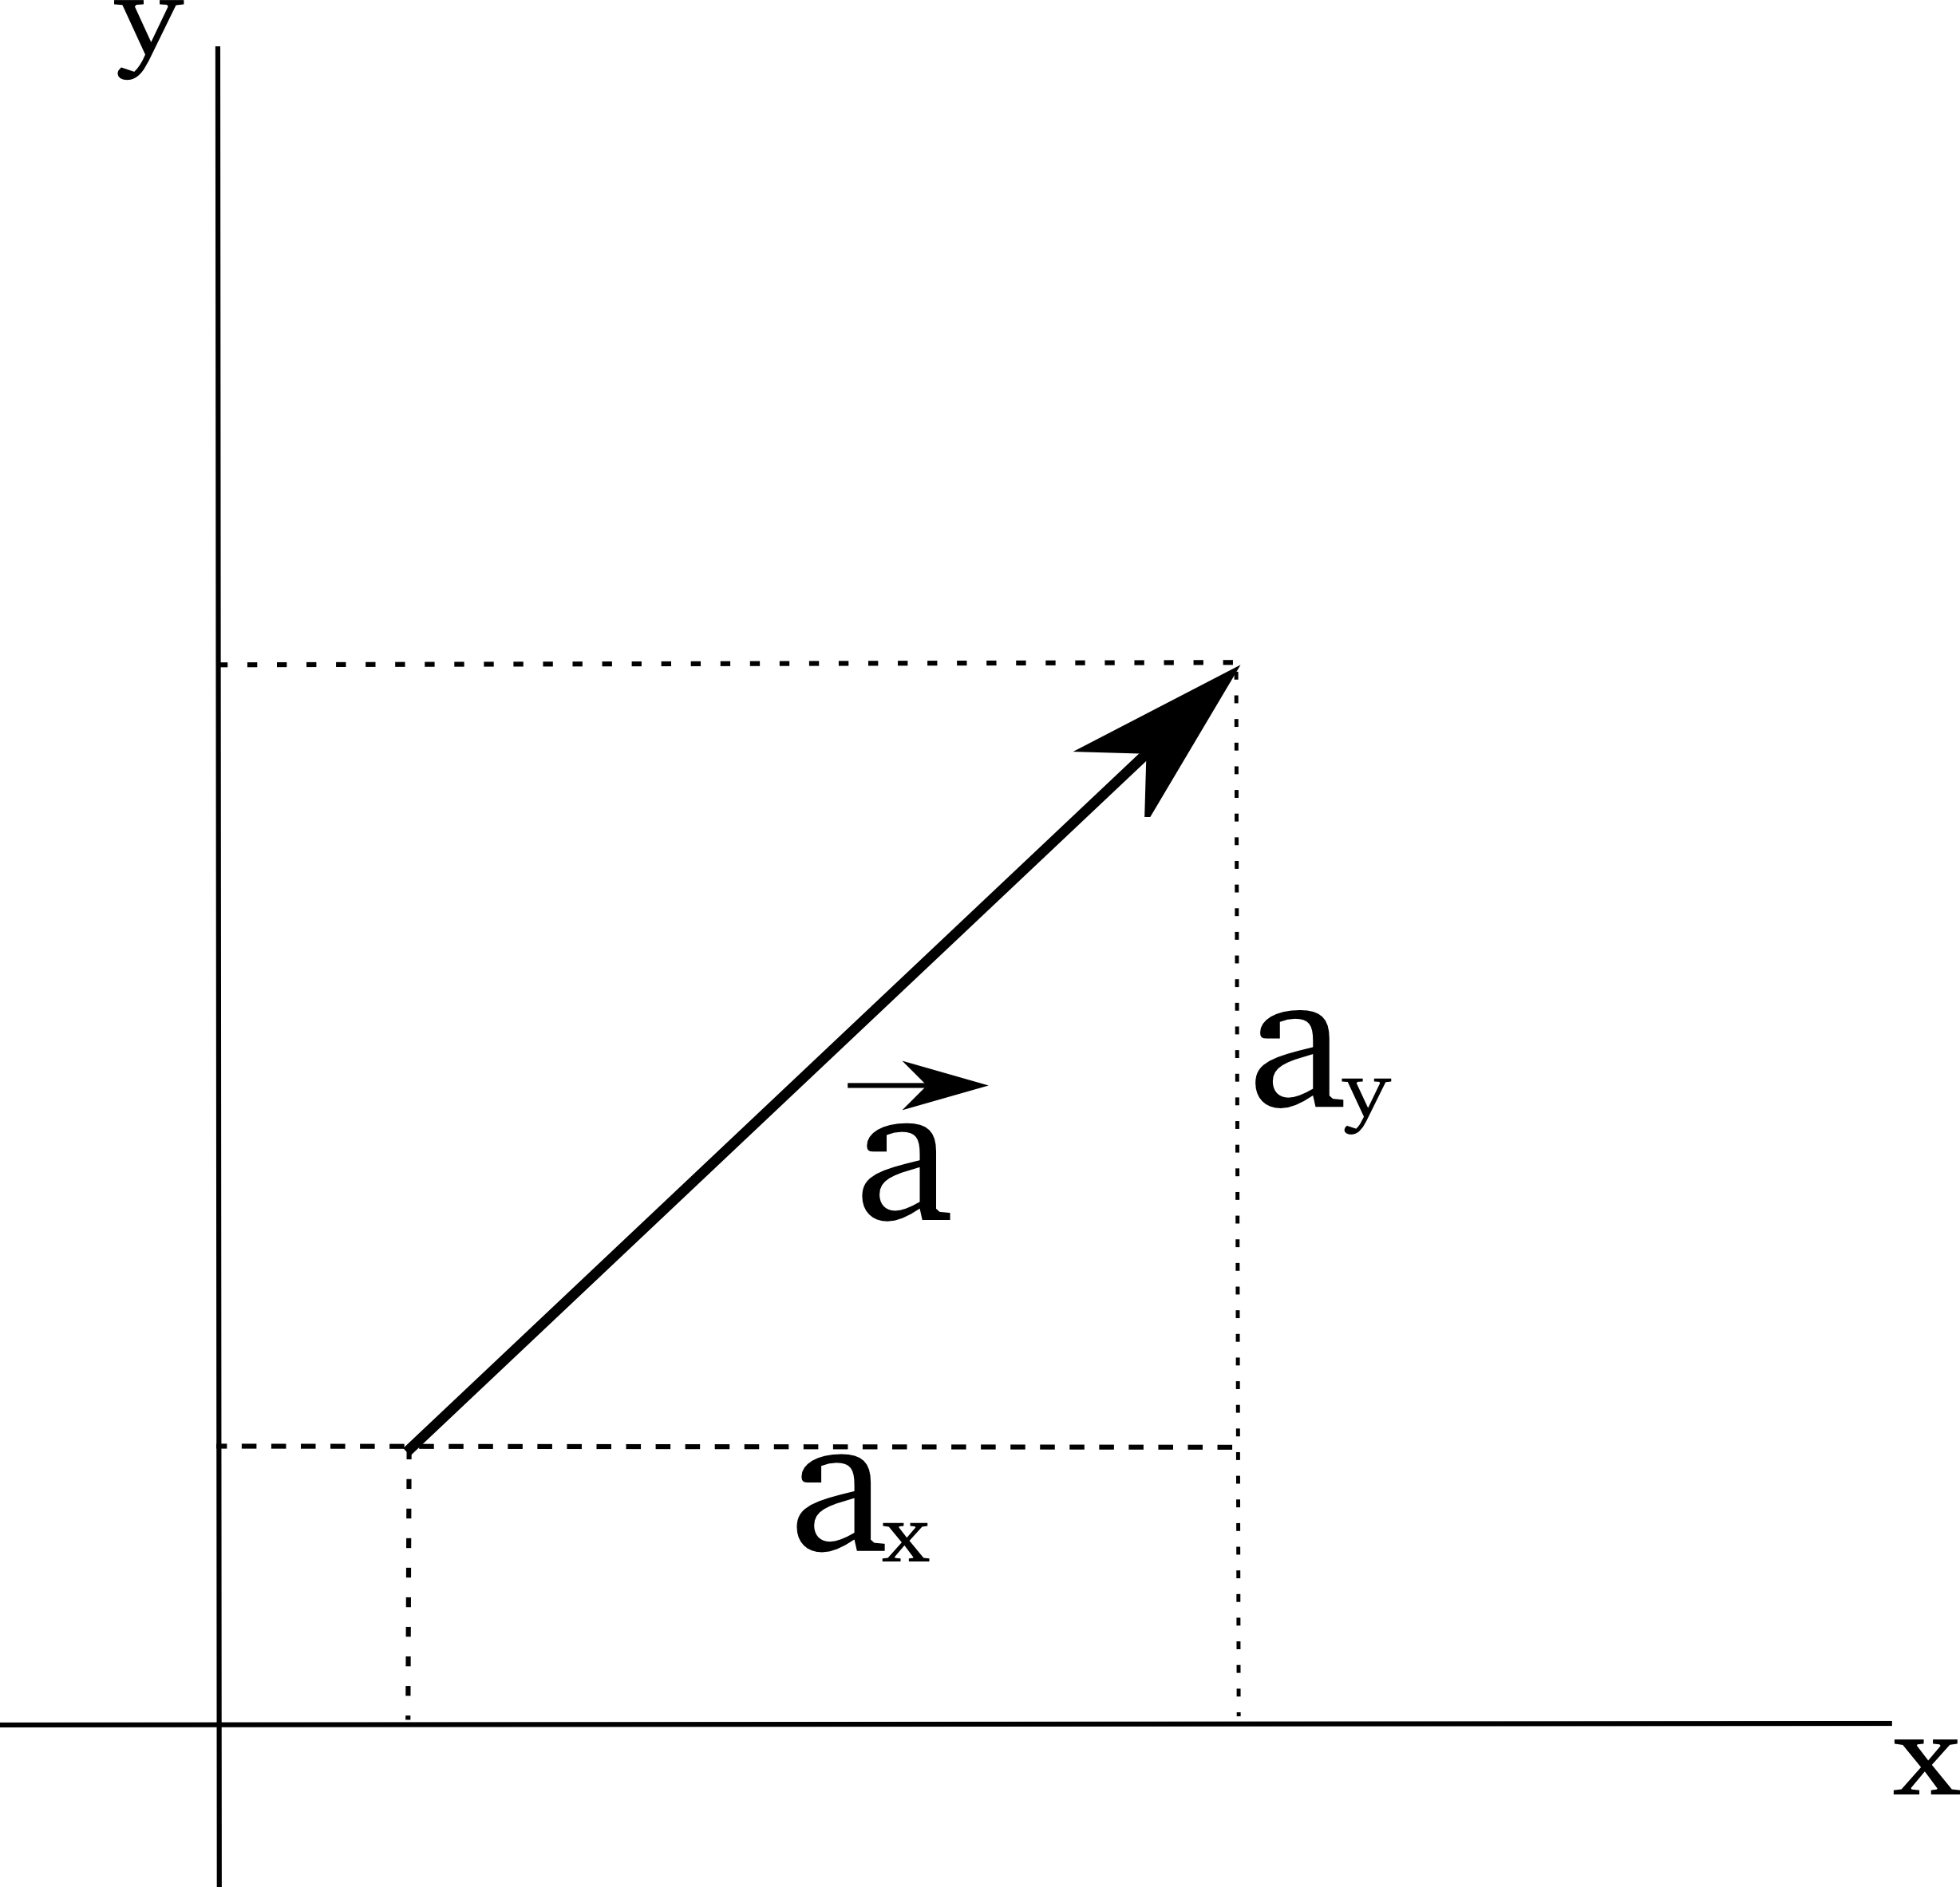
\includegraphics[width=0.6\textwidth]{./immagini/pitagora.png}
 % pitagora.png: 2456x2365 pixel, 556dpi, 11.22x10.81 cm, bb=0 0 318 306
 \caption{Il modulo di un vettore è graficamente la lunghezza dell'ipotenusa di un triangolo rettangolo i cui cateti sono le proiezioni del vettore sugli assi coordinati}
 \label{fig:modulo}
\end{figure}


\begin{figure}[H]
\begin{center}
 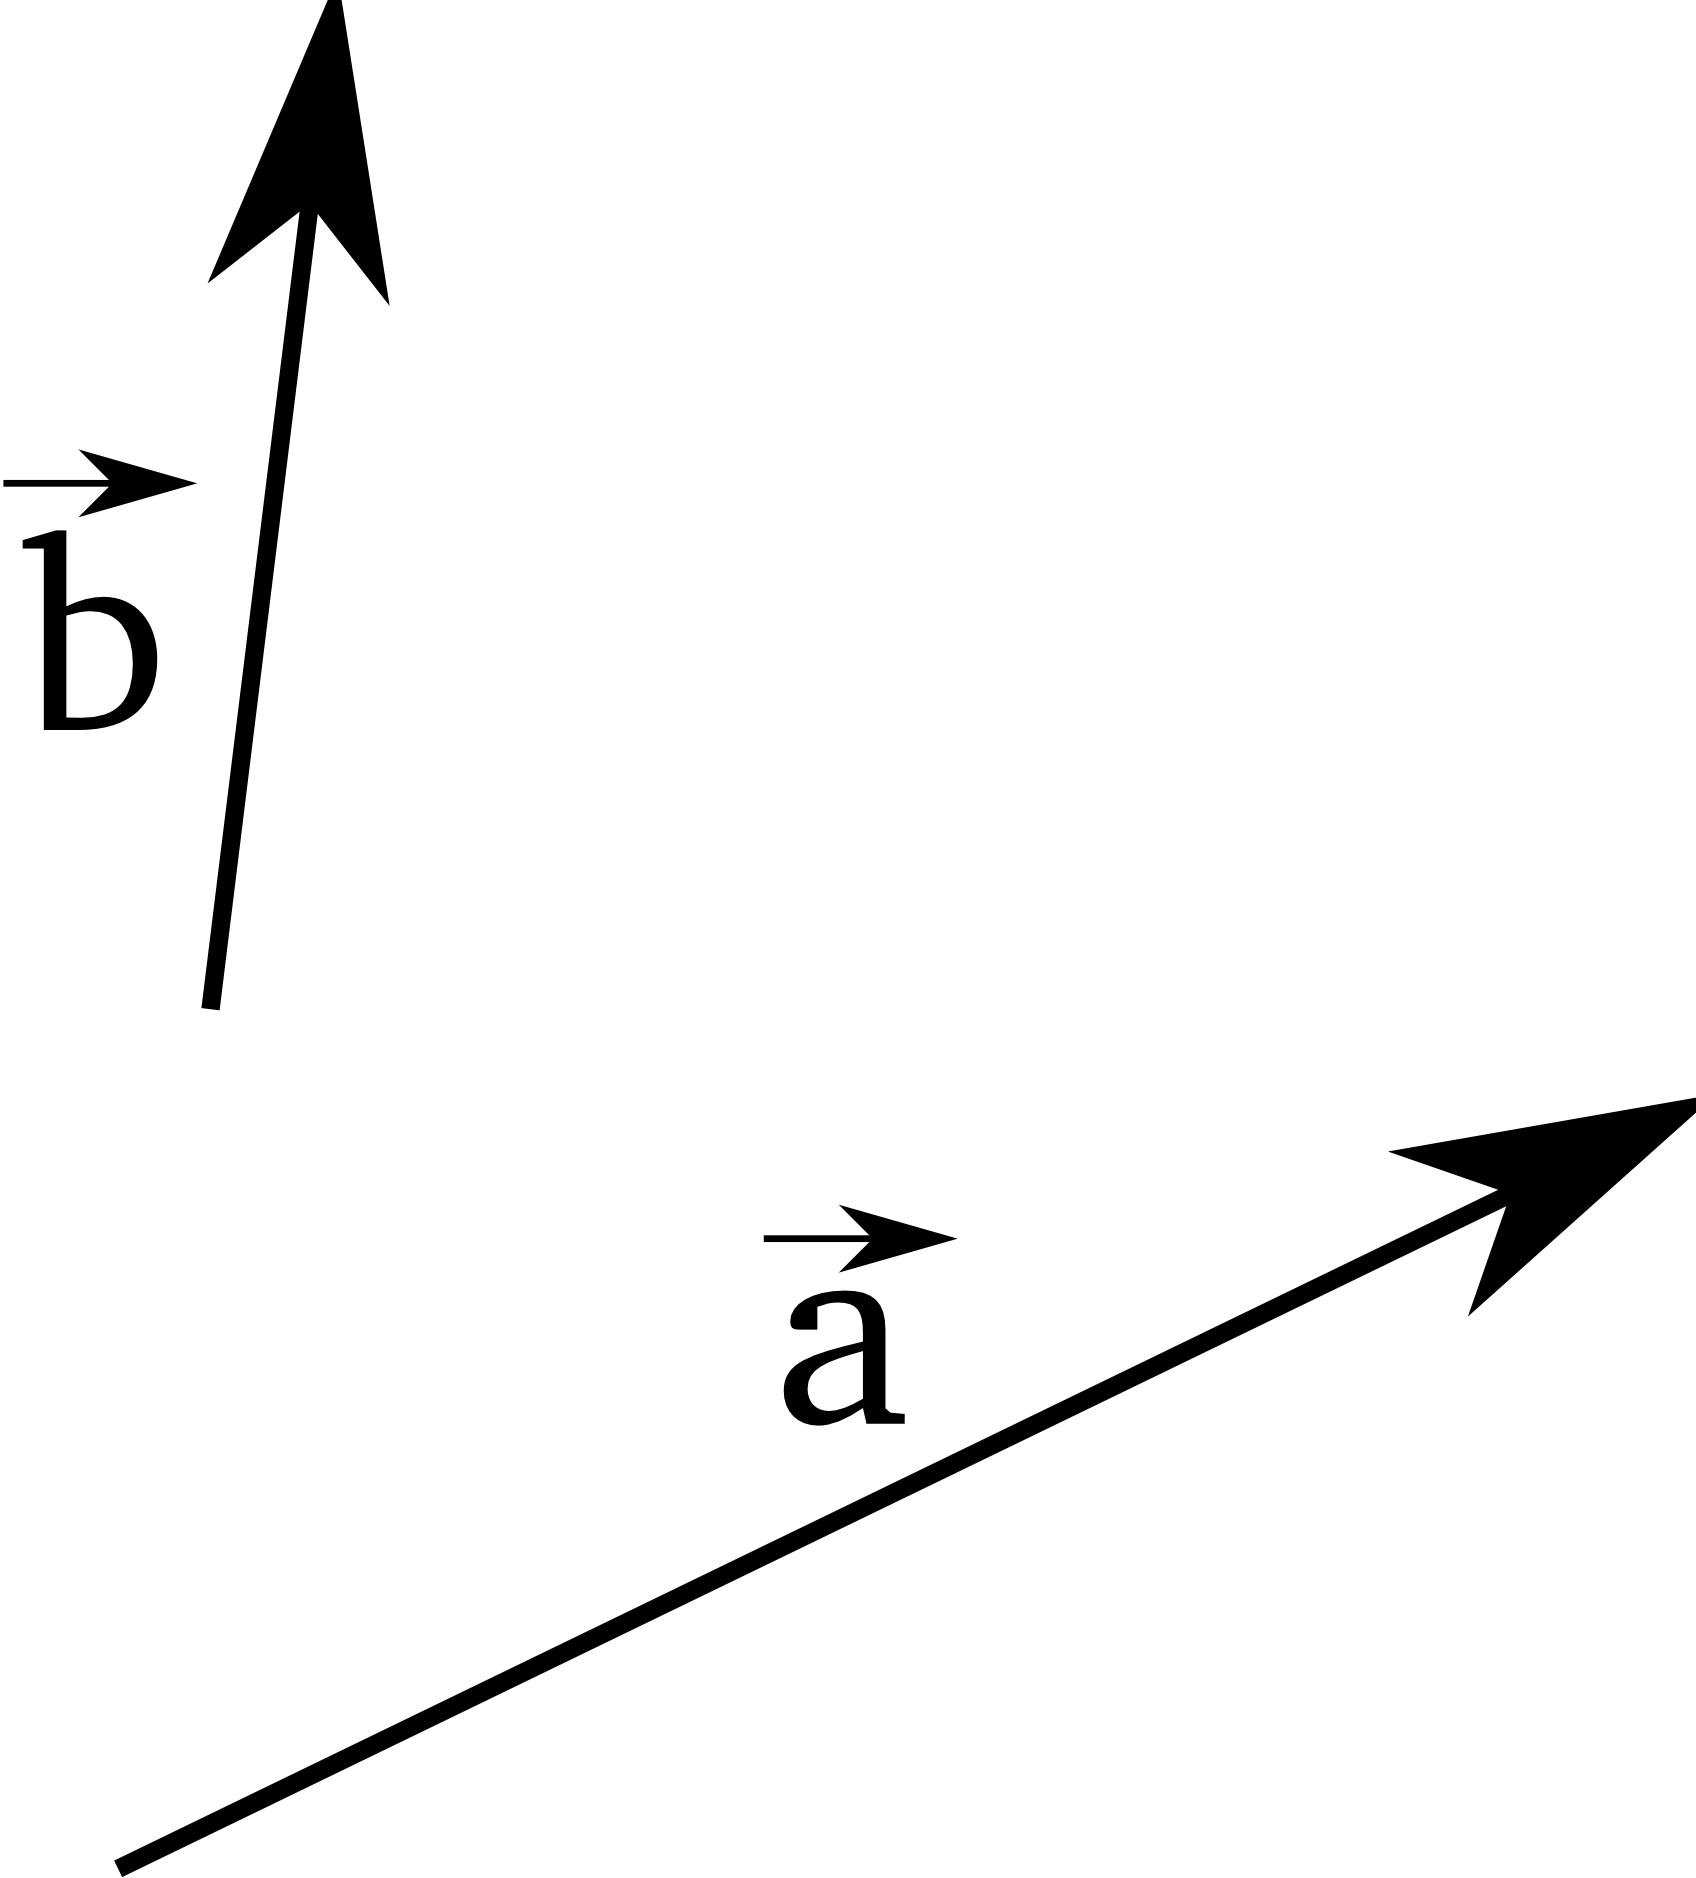
\includegraphics[width=0.3\textwidth]{./immagini/somma_mod1_1.png}
 % somma_mod1_1.png: 1696x1878 pixel, 610dpi, 7.06x7.82 cm, bb=0 0 200 222
 \caption{Sono dati due vettori $\mathbf{a}$ e $\mathbf{b}$}
 \label{fig:somma_base}
\end{center}
\end{figure}

\begin{regola}[ Somma tra vettori]
Dati un vettore $\mathbf{a}$ ed un vettore $\mathbf{b}$ figura [\ref{fig:somma_base}], usiamo la regola del parallelogrammo per calcolare la loro somma. Procederemo nel modo seguente:
\begin{enumerate}
 \item Disegniamo i due vettori in modo che i loro piedi coincidano figura [\ref{fig:mod1_2}]
 \item Tracciamo la retta parallela al vettore $\mathbf{a}$ che passa per il vertice di $\mathbf{b}$ figura [\ref{fig:mod1_3}]
\item Tracciamo la retta parallela al vettore $\mathbf{b}$ che passa per il vertice del vettore $\mathbf{a}$ [\ref{fig:mod1_4}]
\item Disegniamo un terzo vettore con il piede nel punto di incontro dei piedi dei vettori $\mathbf{a}$ e $\mathbf{b}$ e il vertice nel punto di intersezione delle due rette appena tracciate [\ref{fig:mod1_5}]
\end{enumerate}
Possiamo applicare la regola del parallelogrammo in modo simile al precedente facendo coincidere il vertice del vettore $\mathbf{a}$ con il piede del vettore $\mathbf{b}$:
\begin{enumerate}
 \item Disegniamo i due vettori in modo che il vertice di  $\mathbf{a}$ tocchi il piede di $\mathbf{b}$ figura [\ref{fig:mod2_1}]
\item Disegniamo un vettore con il piede coincidente con il piede di $\mathbf{a}$ e il vertice coincidente con il vertice di $\mathbf{b}$ figura [\ref{fig:mod2_2}]
\end{enumerate}
Notiamo come con questo secondo metodo si ottenga il medesimo risultato e che il parallelogrammo ottenuto sia identico a quello precedentemente disegnato figura [\ref{fig:mod2_3}].
\end{regola}

\begin{figure}[H]
 \subfigure[Faccio coincidere i piedi dei vettori]{
   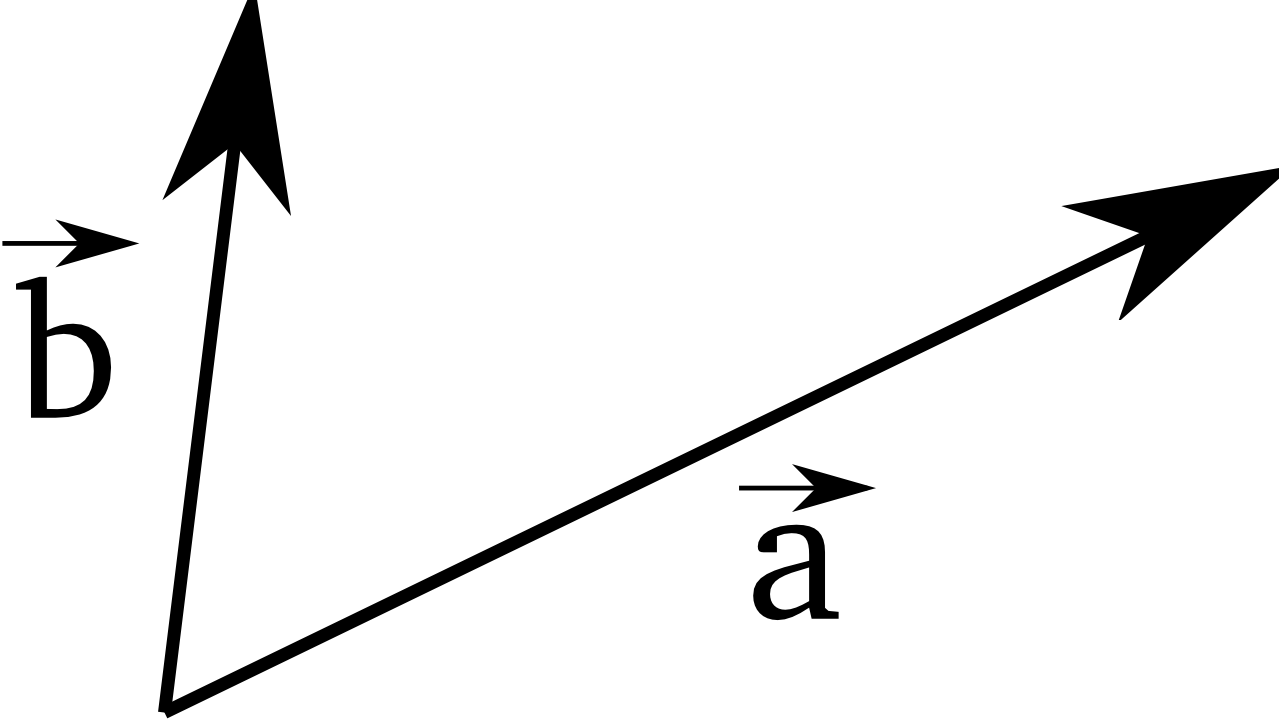
\includegraphics[width=0.3\textwidth]{./immagini/somma_mod1_2.png}
   \label{fig:mod1_2}}
 \subfigure[Traccio la parallela ad $\mathbf{a}$ che passa per il vertice di $\mathbf{b}$]{
  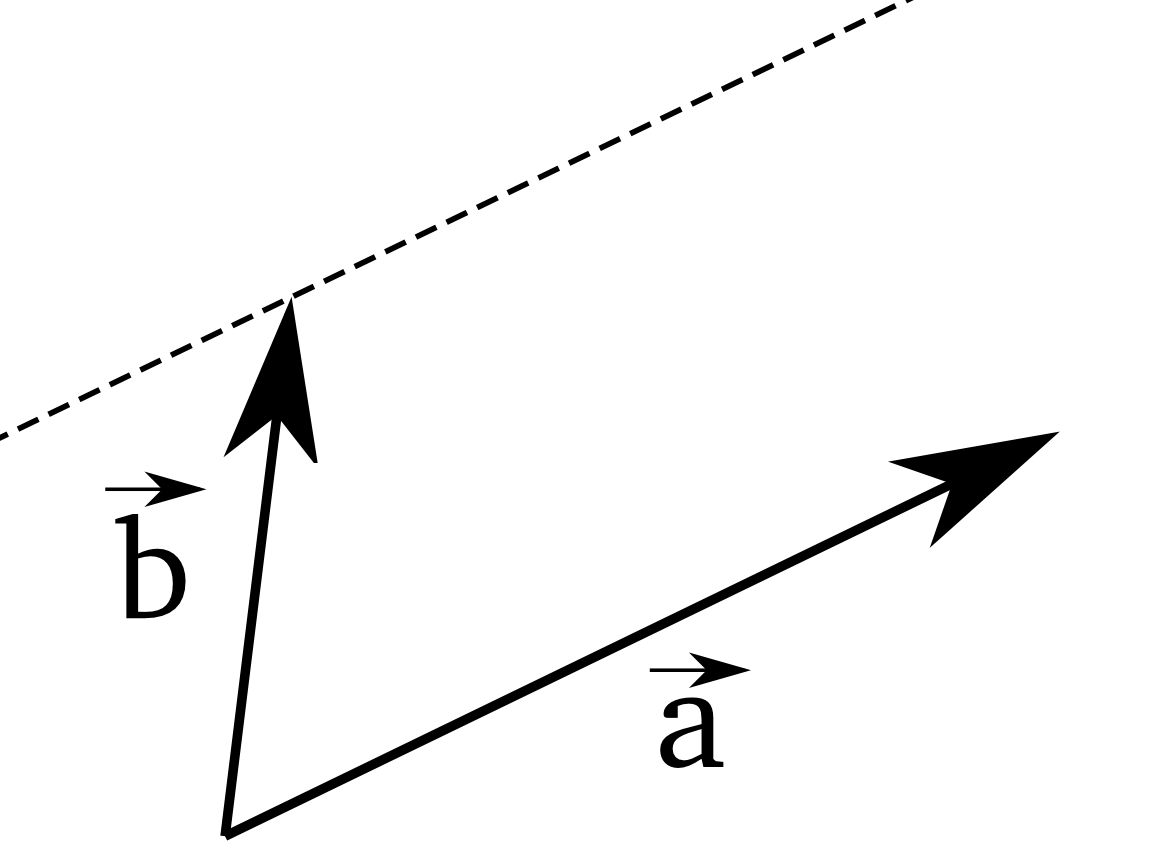
\includegraphics[width=0.3\textwidth]{./immagini/somma_mod1_3.png}
  \label{fig:mod1_3}}
\subfigure[Traccio la parallela a $\mathbf{b}$ che passa per il vertice di $\mathbf{a}$]{
  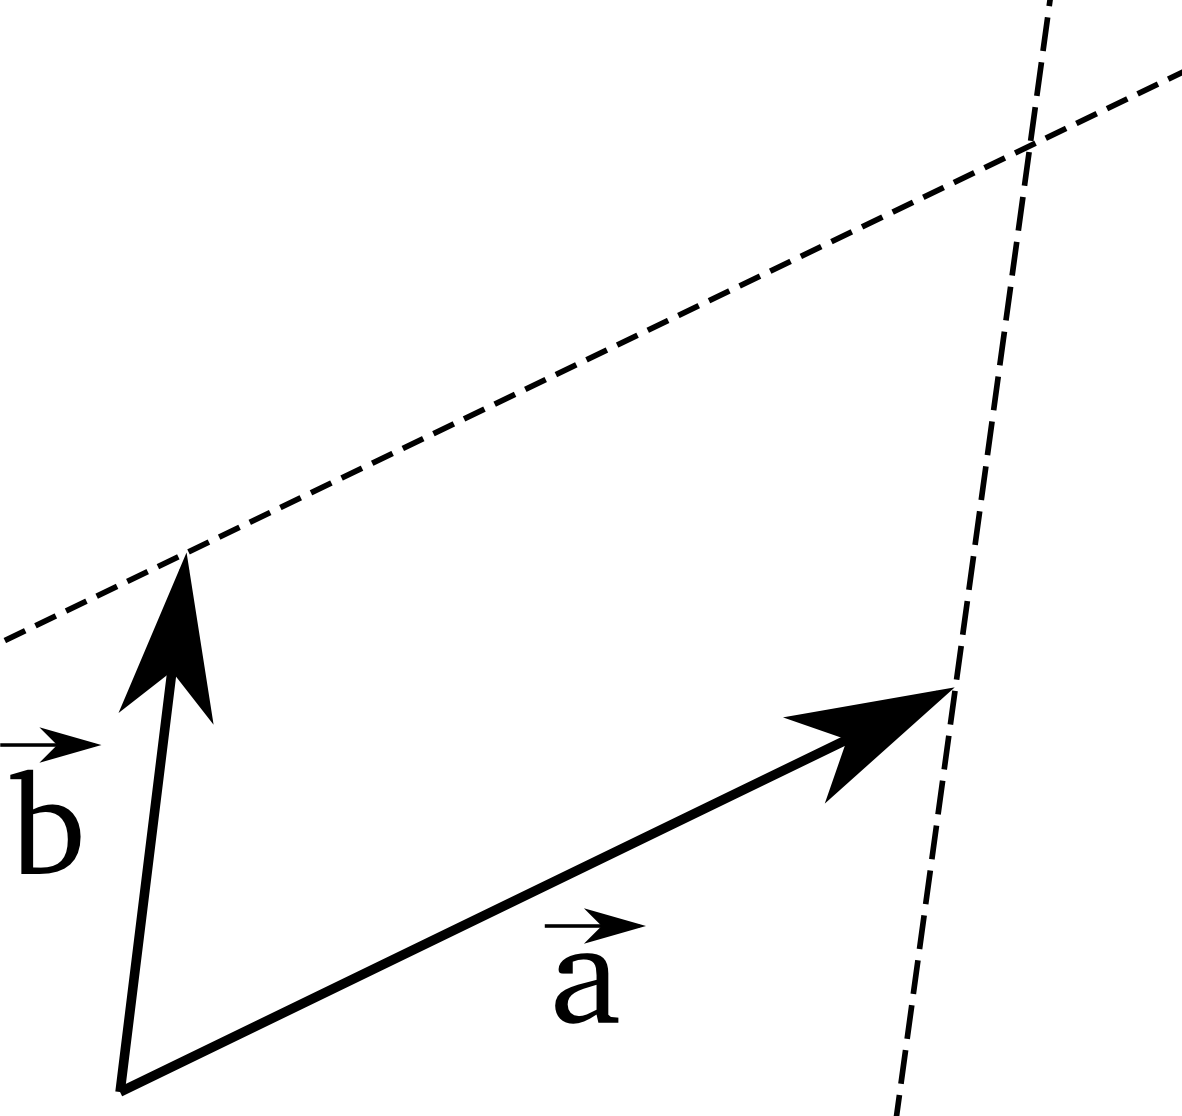
\includegraphics[width=0.3\textwidth]{./immagini/somma_mod1_4.png}
  \label{fig:mod1_4}}
\subfigure[Disegno un terzo vettore con il piede nel punto di incontro dei piedi dei vettori $\mathbf{a}$ e $\mathbf{b}$ e il vertice nel punto di intersezione delle due rette appena tracciate]{
  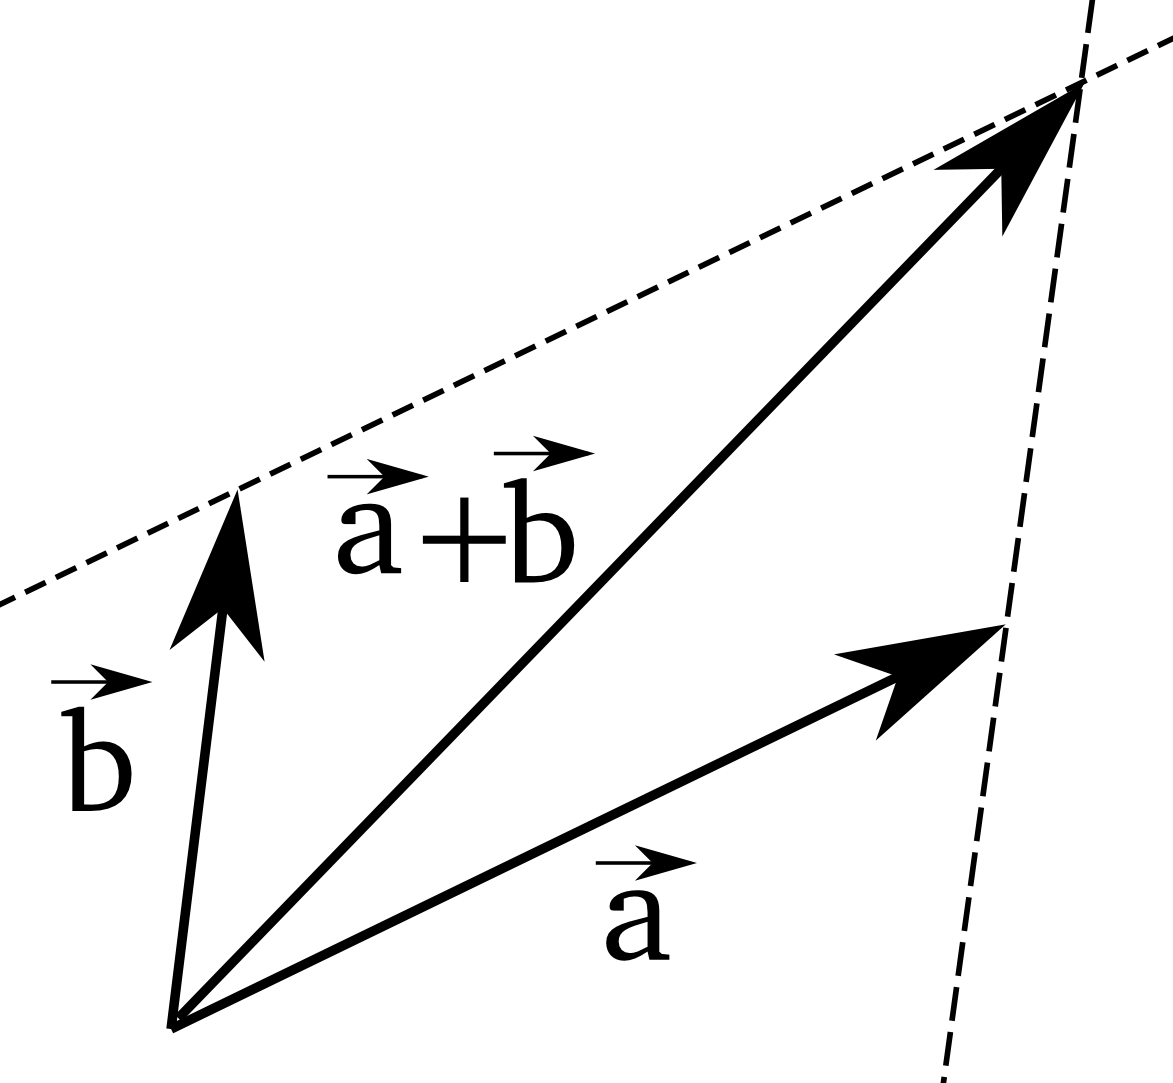
\includegraphics[width=0.3\textwidth]{./immagini/somma_mod1_5.png}
  \label{fig:mod1_5}}
\caption{Somma dei vettori con il metodo del parallelogrammo I}
\end{figure}

\begin{figure}[H]
 \subfigure[Disegniamo i due vettori in modo che il vertice di  $\mathbf{a}$ tocchi il piede di $\mathbf{b}$]{
   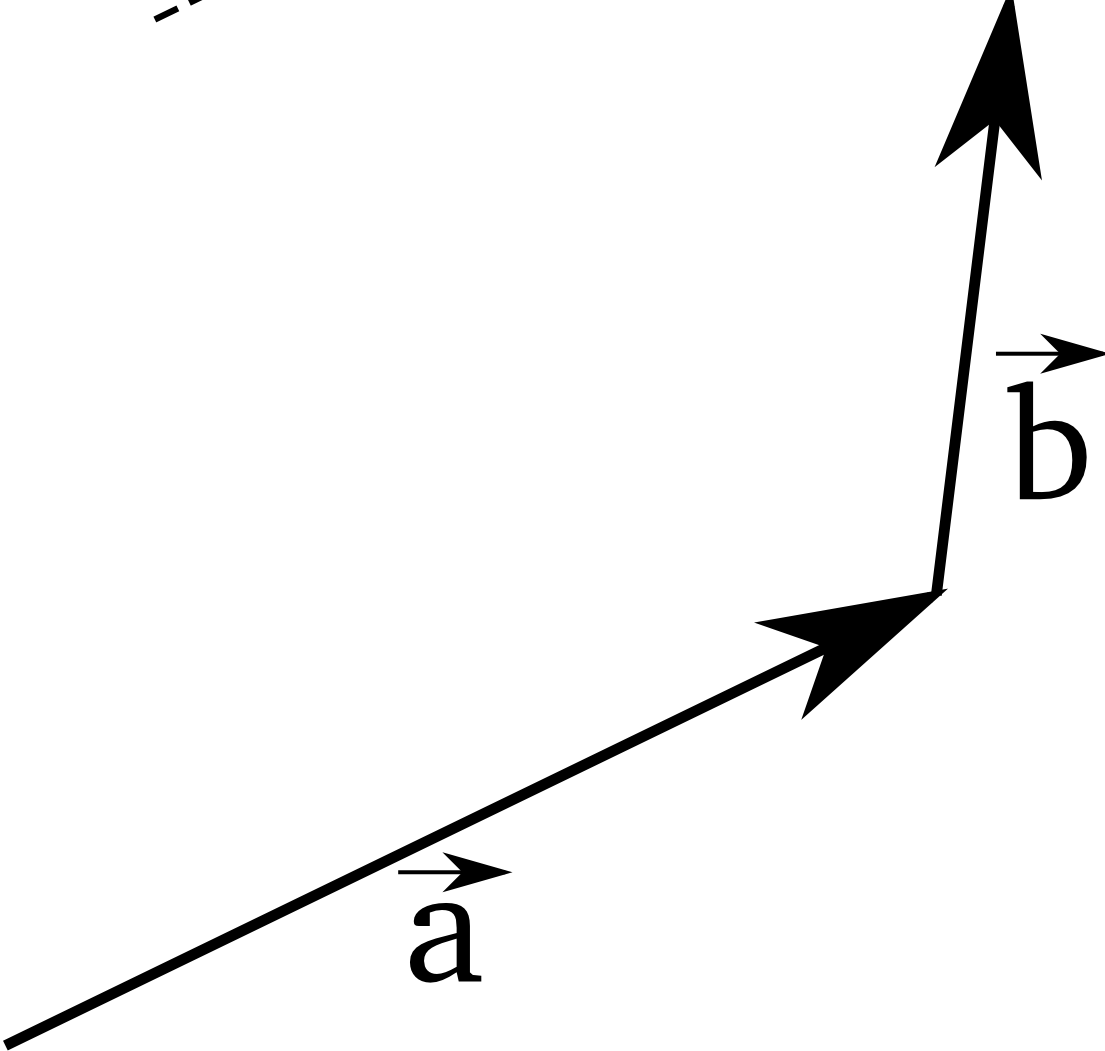
\includegraphics[width=0.3\textwidth]{./immagini/somma_mod2_1.png}
  \label{fig:mod2_1}}
 \subfigure[Disegniamo un vettore con il piede coincidente con il piede di $\mathbf{a}$ e il vertice coincidente con il vertice di $\mathbf{b}$]{
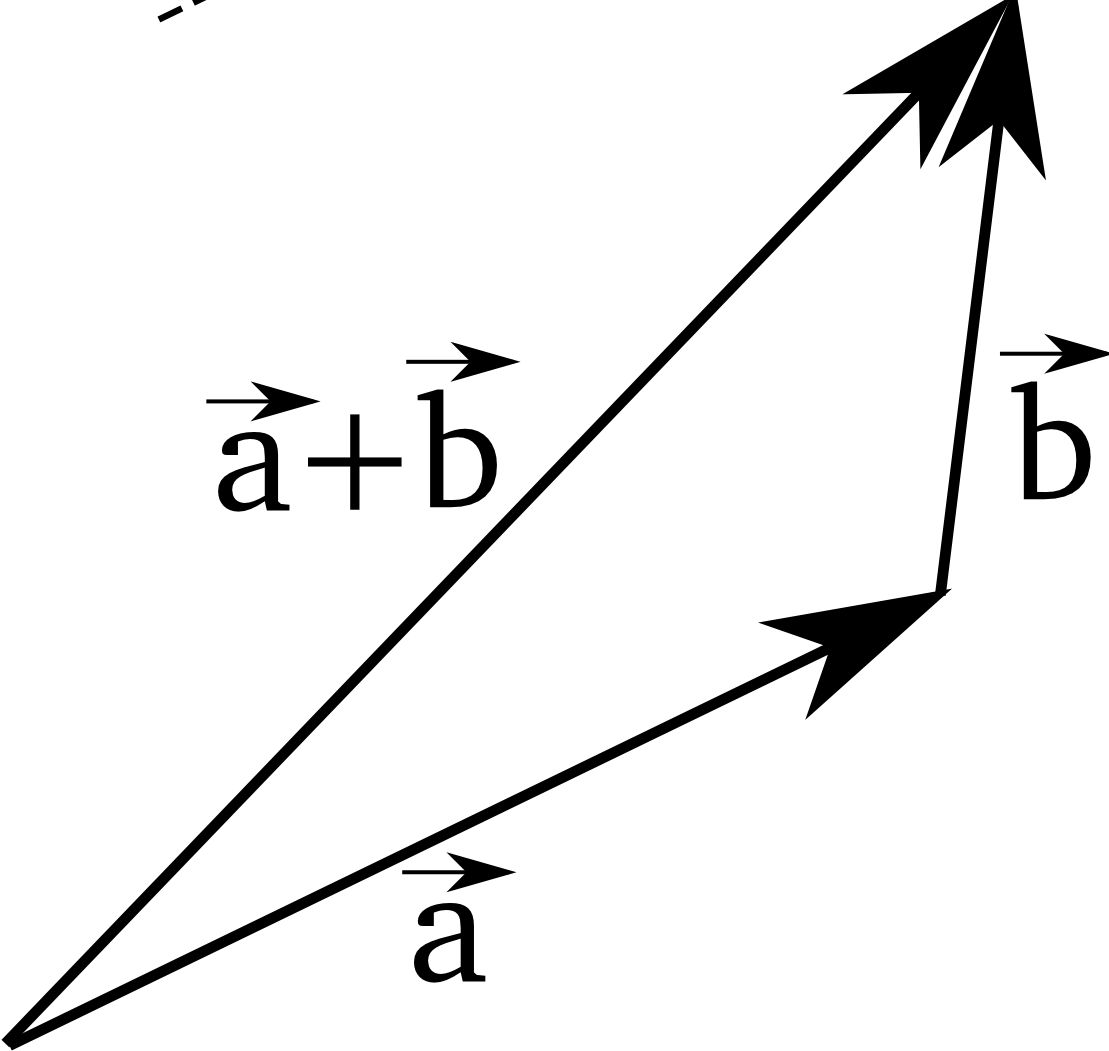
\includegraphics[width=0.3\textwidth]{./immagini/somma_mod2_2.png}
  \label{fig:mod2_2}}
 \subfigure[Notiamo come con questo secondo metodo si ottenga il medesimo risultato e che il parallelogrammo ottenuto sia identico a quello precedentemente disegnato.]{
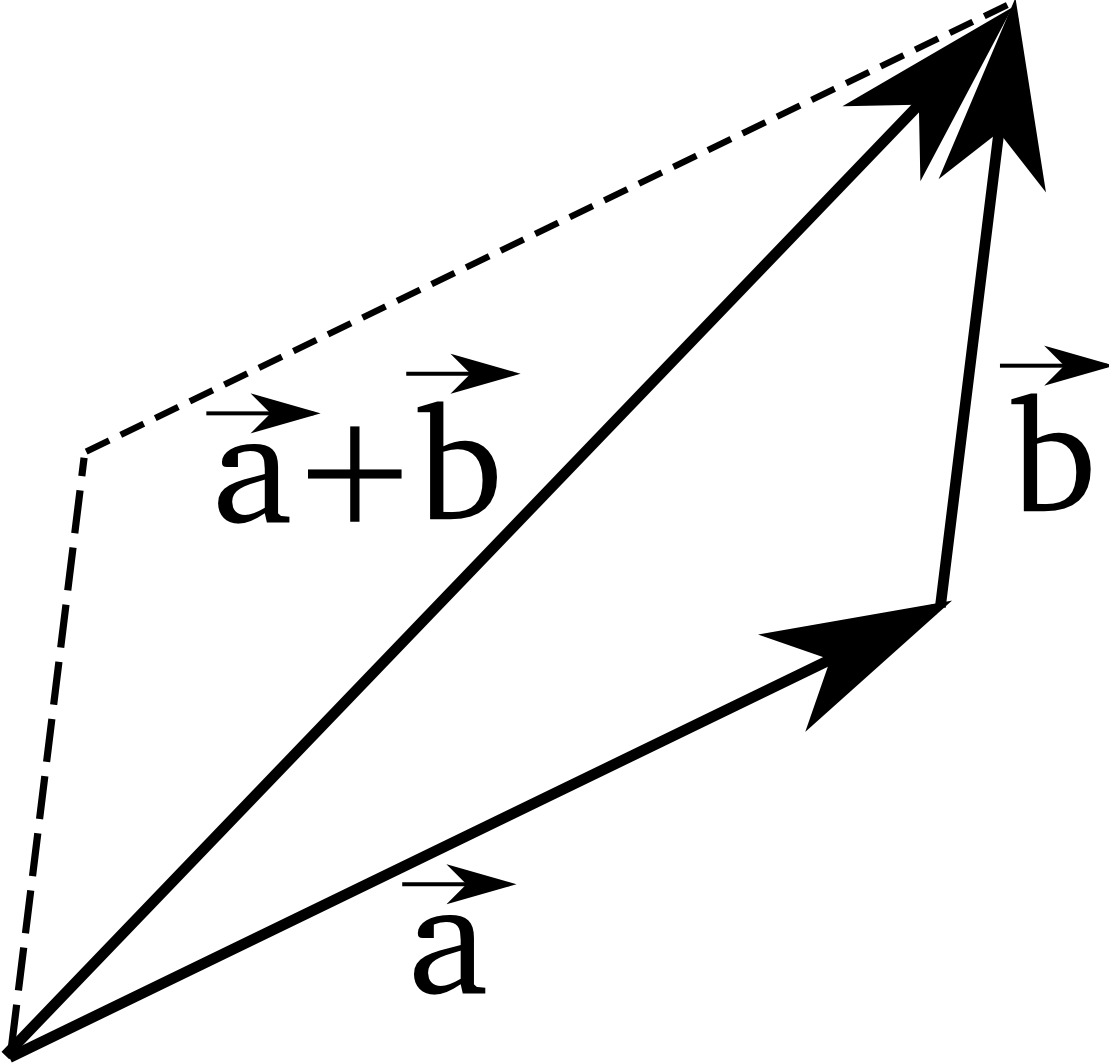
\includegraphics[width=0.3\textwidth]{./immagini/somma_mod2_3.png}
  \label{fig:mod2_3}}
\caption{Somma dei vettori con il metodo del parallelogrammo II}
\end{figure}
\begin{regola}[Prodotto per uno scalare]
Il prodotto di un numero $c$ per un vettore $\mathbf{b}$ è un vettore che ha la stessa direzione del vettore $\mathbf{b}$, modulo pari a $|\mathbf{b}||c|$ figura [\ref{fig:scalare_1}] e verso uguale al verso di $\mathbf{b}$ se $c>0$ verso opposto se $c<0$ figura [\ref{fig:scalare_2}].
\end{regola}
\begin{figure}[H]
\centering
 \subfigure[Se moltiplico per 2 il vettore $\mathbf{b}$ ottengo un vettore con lo stesso verso e la stessa direzione di $\mathbf{b}$ ma con modulo doppio]{
  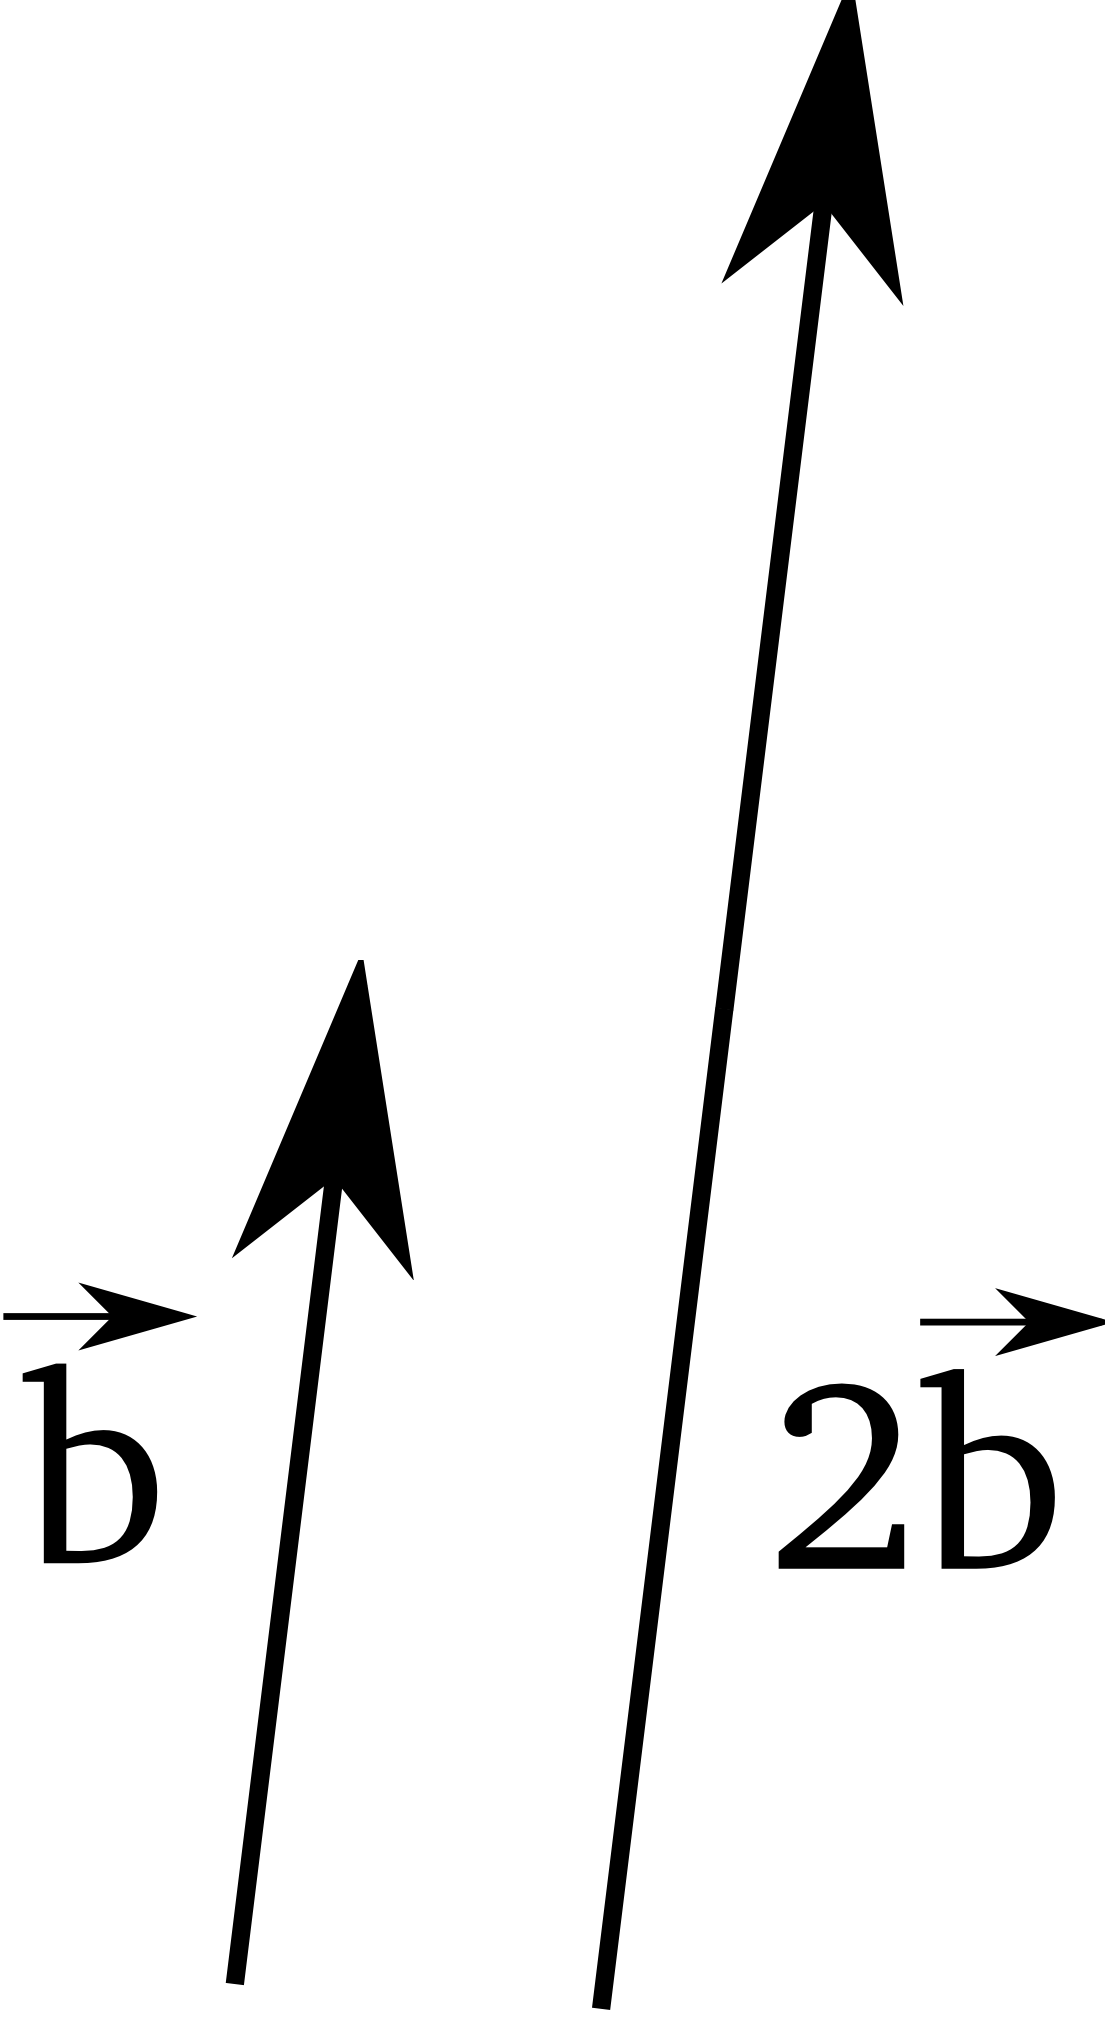
\includegraphics[width=0.3\textwidth]{./immagini/scalare_1.png}
  \label{fig:scalare_1}
  }
 \subfigure[Se moltiplico per $-1$ il vettore $\mathbf{b}$ ottengo un vettore che ha lo stesso modulo la stessa direzione ma verso opposto rispetto al vettore $\mathbf{b}$]{
 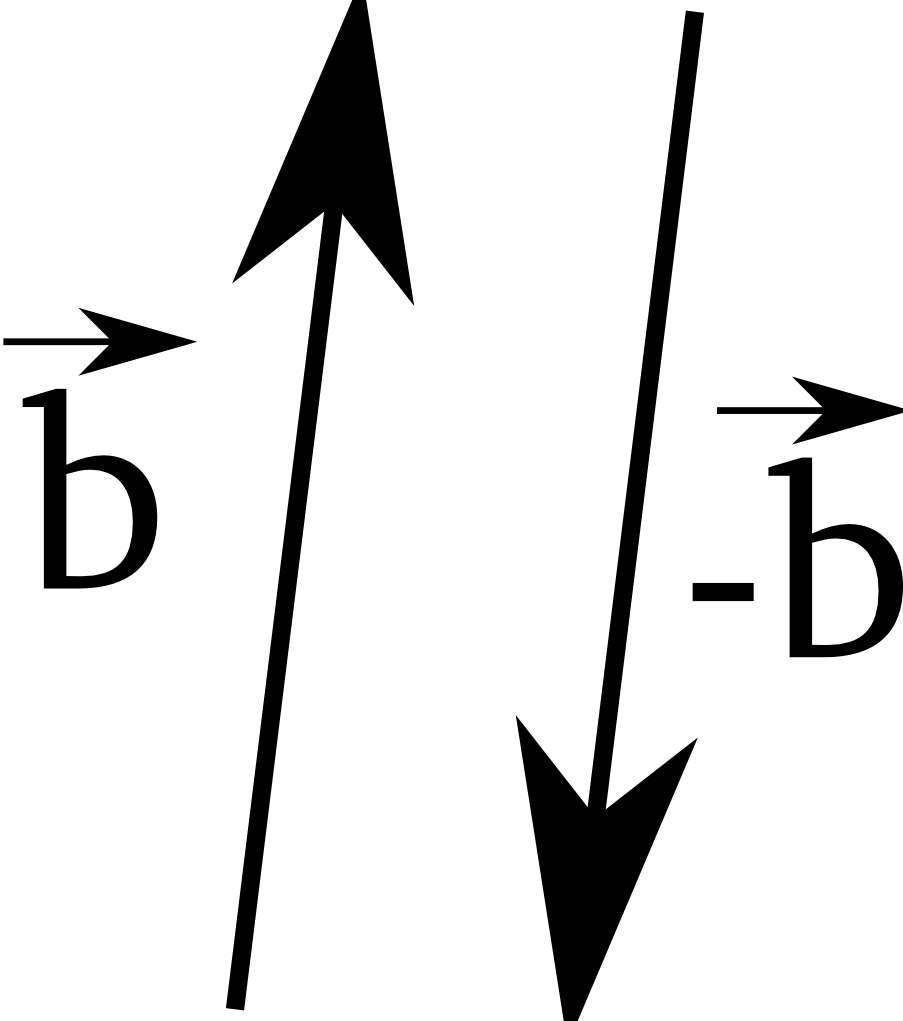
\includegraphics[width=0.3\textwidth]{./immagini/scalare_2.png}
 \label{fig:scalare_2}
}
\caption{Prodotto per uno scalare}
\end{figure}
\begin{regola} [Rappresentazione di un vettore mediante le sue componenti]
 Ogni vettore non nullo può essere espresso come somma di due vettori (in uno spazio bidimensionale, tre in uno spazio tridimensionale) non collineari, usando tale proprietà è possibile rappresentare un vettore bidimensionale qualsiasi coma somma dei versori che identificano gli assi di un sistema cartesiano ortonormale, moltiplicati per dei coefficienti numerici. Tali coefficienti numerici sono le proiezioni del vettore in esame sugli assi coordinati. Chiameremo i versori che definiscono il sistema cartesiano ortonormale  $\hat{\mathbf{x}}$ ed $\hat{\mathbf{y}}$. Le proiezioni nelle direzioni dei versori $\hat{\mathbf{x}}$ ed $\hat{\mathbf{y}}$ sono, detto $\theta$ l'angolo in senso antiorario che il vettore forma con l'asse delle x:
\begin{equation*}
 a_x=|\mathbf{a}|\cos\theta\ a_y=|\mathbf{a}|\sin\theta
\end{equation*}
Il vettore $\mathbf{a}$ scomposto lungo gli assi del sistema di riferimento diventa quindi:
\begin{equation*}
 \mathbf{a}=a_x\hat{\mathbf{x}}+a_y\hat{\mathbf{y}}
\end{equation*}
alternativamente possiamo utilizzare la notazione:
\begin{equation*}
 \mathbf{a}=(a_x,a_y)
\end{equation*}
\end{regola}
\begin{regola}[Differenza di due vettori]
 Per calcolare la differenza tra due vettori $\mathbf{a}$ e $\mathbf{b}$ notiamo che è possibile scrivere:
\begin{equation*}
 \mathbf{a}-\mathbf{b}=\mathbf{a}+(-\mathbf{b})=\mathbf{c}
\end{equation*}
ovvero per sottrarre due vettori è sufficiente sommare ad uno l'opposto dell'altro. Operativamente:
\begin{enumerate}
 \item Calcolo l'opposto del vettore $\mathbf{b}$ figura [\ref{fig:sottr_1}]
\item Faccio coincidere il vertice del vettore $\mathbf{a}$ con il piede del vettore $- \mathbf{b}$ figura [\ref{fig:sottr_2}]
\item Disegno un vettore con il piede coincidente con quello del vettore $\mathbf{a}$ e il vertice coincidente con il vertice del vettore $-\mathbf{b}$ figura [\ref{fig:sottr_3}]
\end{enumerate}
\end{regola}

\begin{figure}[H]
 \subfigure[Calcolo l'opposto del vettore $\mathbf{b}$]{
  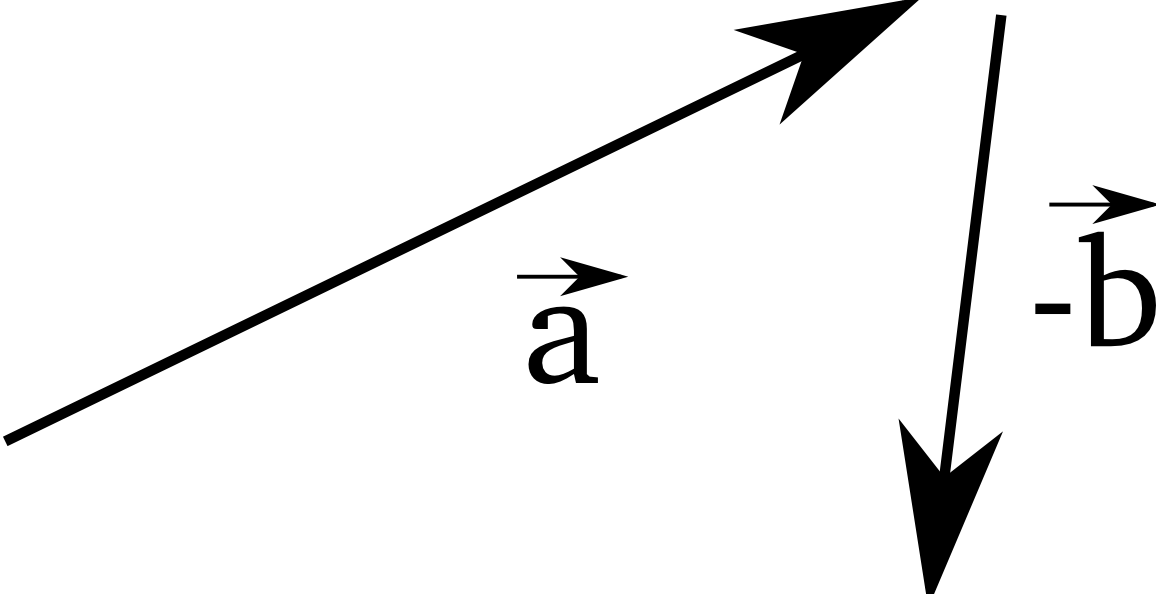
\includegraphics[width=0.3\textwidth]{./immagini/sottr_1.png}
  \label{fig:sottr_1}
}
 \subfigure[Faccio coincidere il vertice del vettore $\mathbf{a}$ con il piede del vettore $- \mathbf{b}$]{
  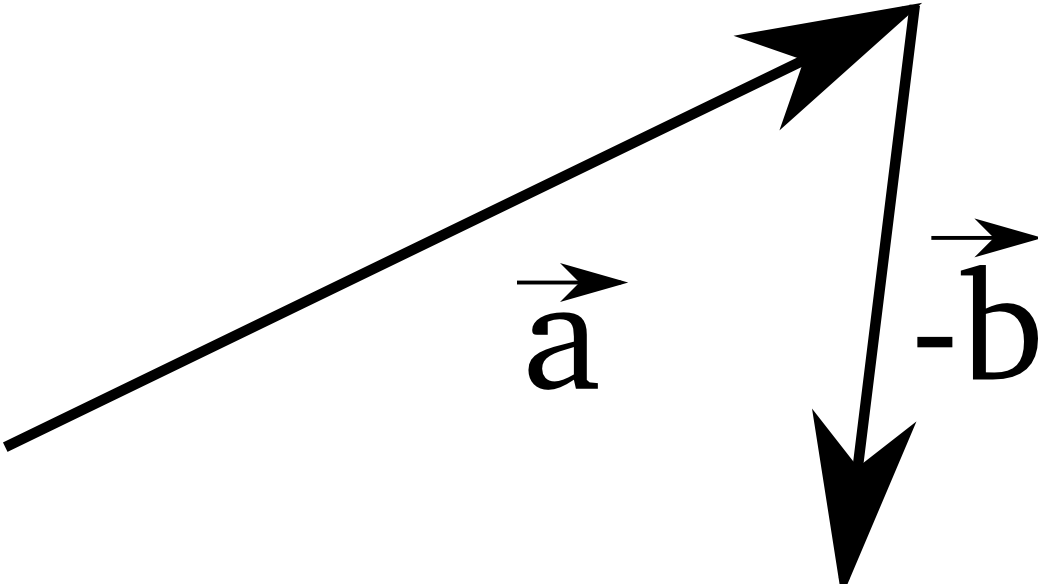
\includegraphics[width=0.3\textwidth]{./immagini/sottr_2.png}
  \label{fig:sottr_2}
}
 \subfigure[Disegno un vettore con il piede coincidente con quello del vettore $\mathbf{a}$ e il vertice coincidente con il vertice del vettore $-\mathbf{b}$]{
   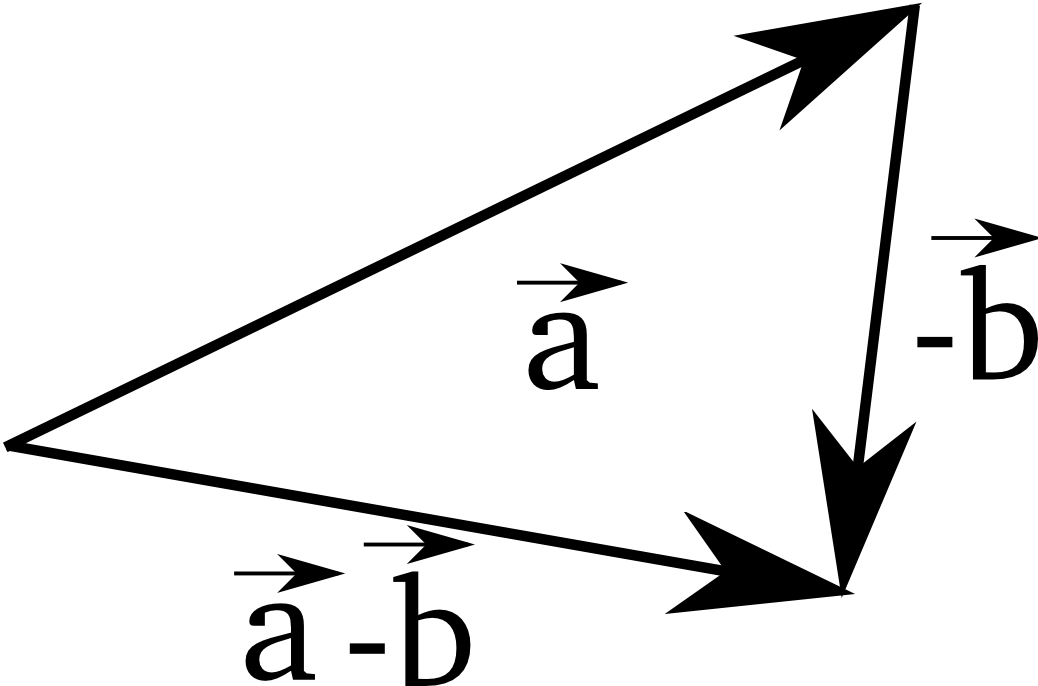
\includegraphics[width=0.3\textwidth]{./immagini/sottr_3.png}
  \label{fig:sottr_3}
}
 \subfigure[Notiamo come si sia sempre usata la regola del parallelogrammo]{ 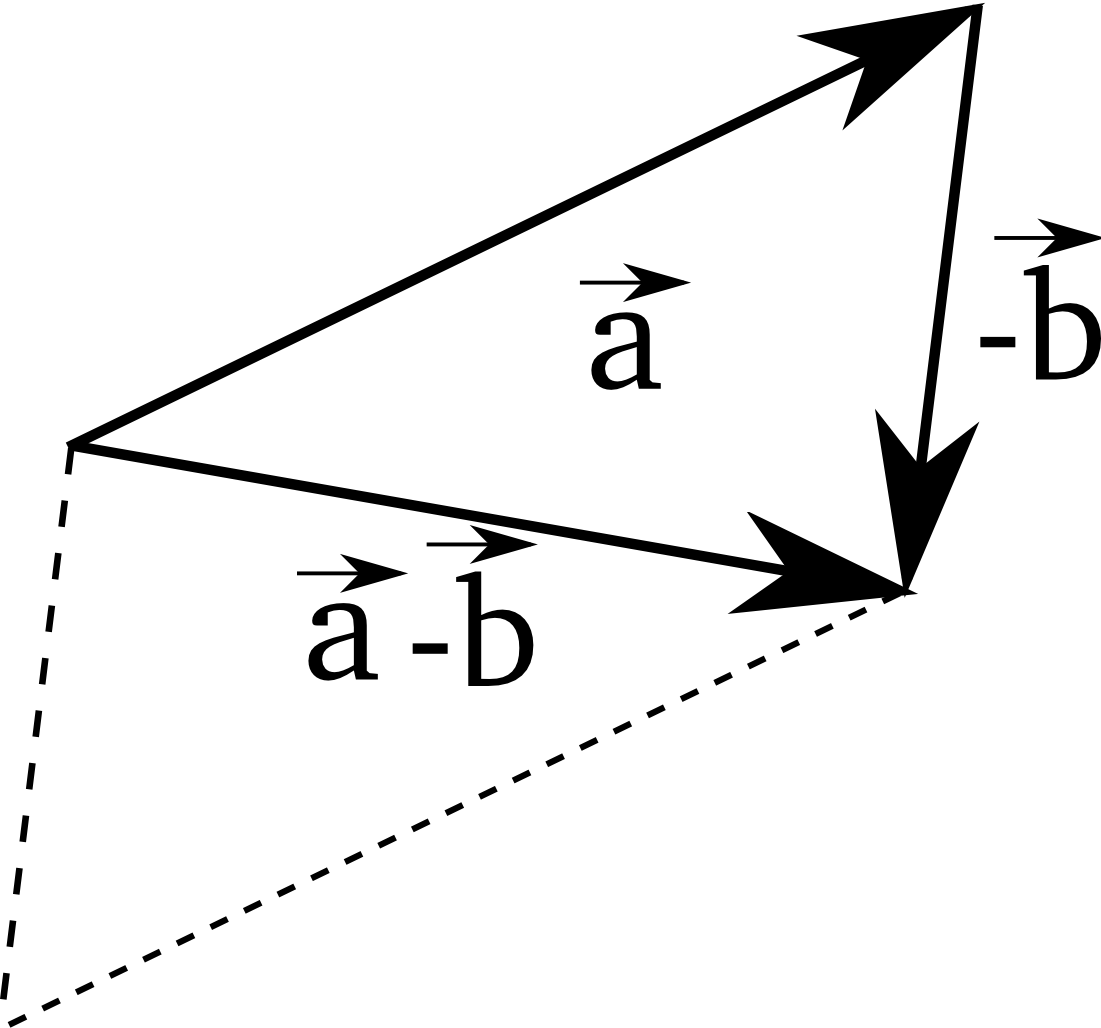
\includegraphics[width=0.3\textwidth]{./immagini/sottr_4.png}
  \label{fig:sottr_4}}
\caption{Sottrazione dei due vettori di figura [\ref{fig:somma_base}]}
\end{figure}



\begin{regola}[Operazioni con i vettori espressi mediante le loro componenti]
La somma di due vettori espressi in componenti è molto semplice, è infatti sufficiente sommare componente per componente. Dati, ad esempio un vettore $\mathbf{a}=(a_x,a_y)$ ed un vettore $\mathbf{b}=(b_x,b_y)$ possiamo trovare un vettore $\mathbf{c}$ somma come:
\begin{equation*}
 \mathbf{c}=\mathbf{a}+\mathbf{b}=(a_x+b_x,a_y+b_y)
\end{equation*}
per calcolare il prodotto per uno scalare è sufficiente moltiplicare entrambe le componenti per lo scalare:
\begin{equation*}
 c\mathbf{a}=(ca_x,ca_y)
\end{equation*}


\end{regola}


\end{document}
